\documentclass[12pt]{article}

\usepackage{amsmath,amsthm,amsfonts,amssymb,amsxtra}
\usepackage{pgf,tikz}
\usetikzlibrary{arrows}
\renewcommand{\theenumi}{(\alph{enumi})} 
\renewcommand{\labelenumi}{\theenumi}

\pagestyle{empty}
\setlength{\textwidth}{7in}
\setlength{\oddsidemargin}{-0.5in}
\setlength{\topmargin}{-1.0in}
\setlength{\textheight}{9.5in}

\theoremstyle{definition}
\newtheorem{problem}{Problem}

\begin{document}

\noindent{\large\bf MATH 241}\hfill{\large\bf Exam \#2}\hfill{\large\bf
  Spring 2017}\hfill{\large\bf Page 1/5}\hrule

\bigskip
\begin{center}
  \begin{tabular}{|ll|}
    \hline & \cr
    {\bf Name: } & \makebox[12cm]{\hrulefill}\cr & \cr
    {\bf VIP ID:} & \makebox[12cm]{\hrulefill}\cr & \cr
    \hline
  \end{tabular}
\end{center}
\begin{itemize}
\item Write your name and your VIP ID in the space provided above.
\item The test has five (5) pages, including this one.
\item Enter your answer in the box(es) provided.
\item You must show sufficient work to justify all answers unless
  otherwise stated in the problem.  Correct answers with inconsistent
  work may not be given credit.
\item Credit for each problem is given in parentheses at the right of
  the problem number.
\item No books, notes or calculators may be used on this test.
\end{itemize}
\hrule

\begin{center}
  \begin{tabular}{|c|c|c|}
    \hline
    &&\cr
    {\large\bf Page} & {\large\bf Max.~points} & {\large\bf Your points} \cr
    &&\cr
    \hline
    &&\cr
    {\Large 2} & \Large 20 & \cr
    &&\cr
    \hline
    &&\cr
    {\Large 3} & \Large 30 & \cr
    &&\cr
    \hline
    &&\cr
    {\Large 4} & \Large 20 & \cr
    &&\cr
    \hline
    &&\cr
    {\Large 5} & \Large 30 & \cr
    &&\cr
    \hline\hline
    &&\cr
    {\large\bf Total} & \Large 100 & \cr
    &&\cr
    \hline
  \end{tabular}
\end{center}
\newpage

%%%%%%%%%%%%%%%%%%%%%%%%%%%%%%%%%%%%% Page 2
\noindent{\large\bf MATH 241}\hfill{\large\bf Exam \#2}\hfill{\large\bf
  Spring 2017}\hfill{\large\bf Page 2/5}\hrule

\bigskip
\begin{problem}[10 pts] 
Find (and sketch) the domain of $f(x,y)=\dfrac{\sqrt{4-x^2}}{y^2+3}$

\begin{tikzpicture}
\draw [white] (-3.5,-3.5) rectangle (3.5,3.5);
\draw [<->, ultra thick] (-3.5,0) -- (3.5,0);
\draw [<->, ultra thick] (0,-3.5) -- (0,3.5);
\draw[step=0.5,black,thin] (-3.25, -3.25) grid (3.25, 3.25);
\draw (4.5, -3.5) -- (4.5, 3.5);
\draw (6.5,3) node {Show work here:};
\end{tikzpicture}
\begin{flushright}
  \begin{tikzpicture}
    \draw (-8.0cm,2.1cm) node {domain:};
    \draw (-7cm,1.4cm) rectangle (5cm,2.8cm);
  \end{tikzpicture}
\end{flushright}
\end{problem}
\hrule
\begin{problem}[10 pts---5 points each part]
For the function $f(x,y) = \sqrt{y-x^2+x}$.
\begin{enumerate}
  \item Sketch the level lines $f(x,y)=k$ for $k=-1,0,1,2$ \newline \noindent(whenever the equations make sense)
  \item Use the previous information to compute the range of the function $f$.
\end{enumerate}

\begin{tikzpicture}
\draw [white] (-3.5,-3.5) rectangle (3.5,3.5);
\draw [<->, ultra thick] (-3.5,0) -- (3.5,0);
\draw [<->, ultra thick] (0,-3.5) -- (0,3.5);
\draw[step=0.5,black,thin] (-3.25, -3.25) grid (3.25, 3.25);
\draw (4.5, -3.5) -- (4.5, 3.5);
\draw (6.5, 3) node {Show work here:};
\end{tikzpicture}
\begin{flushright}
  \begin{tikzpicture}
    \draw (-1.0cm,2.1cm) node {range:};
    \draw (-0cm,1.4cm) rectangle (5cm,2.8cm);
  \end{tikzpicture}
\end{flushright}
\end{problem}
\newpage

%%%%%%%%%%%%%%%%%%%%%%%%%%%%%%%%%%%%% Page 3
\noindent{\large\bf MATH 241}\hfill{\large\bf Exam \#2}\hfill{\large\bf
  Spring 2017}\hfill{\large\bf Page 3/5}\hrule

\bigskip
\begin{problem}[10 pts] Find the partial derivatives $\frac{\partial f}{\partial x}$ and $\frac{\partial f}{\partial y}$ of the function $f(x,y) = \dfrac{xy^2}{y+2x}$.
\vspace{3.5cm}
\begin{flushright}
  \begin{tikzpicture}
    \draw (-11.8cm, 0.5cm) node {$\dfrac{\partial f}{\partial x} = $};
    \draw (-11cm,-0.2cm) rectangle (-4cm,1.2cm);
    \draw (-2.8cm, 0.5cm) node {$\dfrac{\partial f}{\partial x} = $};
    \draw (-2cm, -0.2cm) rectangle (5cm,1.2cm);
  \end{tikzpicture}
\end{flushright}
\end{problem}
\hrule
\begin{problem}[10 pts]
Compute the directional derivative $D_{\boldsymbol{v}}f(0,\pi)$ for the function $f(x,y) = e^x \cos(xy^2-2y)$ and the direction of the vector $\boldsymbol{v} = \boldsymbol{i} + \boldsymbol{j}$.
\vspace{4.5cm}
\begin{flushright}
  \begin{tikzpicture}
    \draw (-1.2cm,0.5cm) node {$D_{\boldsymbol{v}} f(0,\pi) = $};
    \draw (0cm,-0.2cm) rectangle (5cm,1.2cm);
  \end{tikzpicture}
\end{flushright}
\end{problem}
\hrule
\begin{problem}[10 pts---5 pts each]
Compute the following limits.  If necessary, re-write the fraction first.
\begin{enumerate}
  \item $\displaystyle{\lim_{(x,y) \to (0,0)} \cos \frac{x^2+y^3}{x+y+1}} = $
  \vspace{1cm}
  \item $\displaystyle{\lim_{(x,y). \to (2,0)} \frac{\sqrt{2x-y}-2}{2x-y-4}} = $ 
\end{enumerate}
\end{problem}
\newpage

%%%%%%%%%%%%%%%%%%%%%%%%%%%%%%%%%%%%% Page 4
\noindent{\large\bf MATH 241}\hfill{\large\bf Exam \#2}\hfill{\large\bf
  Spring 2017}\hfill{\large\bf Page 4/5}\hrule

\bigskip

\begin{problem}[10 pts---5 pts each]
Limits that do not exist:
\begin{enumerate}
  \item By considering different paths of approach, show that $\displaystyle{\lim_{(x,y) \to (0,0)} \frac{x^2-y}{x-y}}$ does not exist.
  \vspace{4.5cm}
  \item By changing the limit to polar coordinates, show that $\displaystyle{\lim_{(x,y) \to (0,0)} \frac{x-y}{x+y}}$ does not exist.
  \vspace{4.5cm}
\end{enumerate}
\end{problem}
\hrule
\begin{problem}[10 pts]
At what points does the vector function $\boldsymbol{r}(t) = \langle \sin t, \cos t, t \rangle$ intersect the sphere $x^2+y^2+z^2 = 5$?
\vspace{7cm}
\begin{flushright}
  \begin{tikzpicture}
    \draw (-5.8cm, 0.5cm) node {points: };
    \draw (-5cm, -0.2cm) rectangle (5cm,1.2cm);
  \end{tikzpicture}
\end{flushright}
\end{problem}
\newpage

%%%%%%%%%%%%%%%%%%%%%%%%%%%%%%%%%%%%% Page 5
\noindent{\large\bf MATH 241}\hfill{\large\bf Exam \#2}\hfill{\large\bf
  Spring 2017}\hfill{\large\bf Page 5/5}\hrule

\bigskip
\begin{problem}[10 pts]
Find the length $\ell$ of the curve $\boldsymbol{r}(t) = \boldsymbol{i} + t^2 \boldsymbol{j} + t^3 \boldsymbol{k}$ for $0 \leq t \leq 1$.
\vspace{9cm}
\begin{flushright}
  \begin{tikzpicture}
    \draw (-0.5cm,0.5cm) node {$\ell = $};
    \draw (0cm,-0.2cm) rectangle (5cm,1.2cm);
  \end{tikzpicture}
\end{flushright}
\end{problem}
\hrule
\begin{problem}[20 pts]
Compute the curvature $\kappa(t)$ of the vector function $\boldsymbol{r}(t) = \langle 4\cos t, 4\sin t, 3t \rangle$.
\vspace{9cm}
\begin{flushright}
  \begin{tikzpicture}
    \draw (-0.8cm,0.5cm) node {$\kappa(t) = $};
    \draw (0cm,-0.2cm) rectangle (5cm,1.2cm);
  \end{tikzpicture}
\end{flushright}
\end{problem}
\end{document}
